\documentclass{article}



\usepackage[utf8]{inputenc}
\usepackage{graphicx}		% Graphics.
\usepackage{color}
\usepackage[english]{babel}
\usepackage{float}
\usepackage{subcaption}
\usepackage{xfrac}
\usepackage{matlab-prettifier}
\usepackage{amsmath}    
\usepackage{amssymb}
\usepackage{siunitx}
\usepackage{chemformula}
\usepackage{physics}
\usepackage{siunitx}
\usepackage[final]{pdfpages}
\usepackage{pdflscape}

% Force centering below figures.
\usepackage[justification=centering]{caption}

% Create a separate table for the appendix.
\usepackage[toc]{appendix}
\usepackage{etoc}

% Table of Content has fast links to sections.
\usepackage{hyperref}

% Remove dots in table of contents.
\usepackage[titles]{tocloft}
\renewcommand{\cftdot}{}

% Page style.
\usepackage[top=2cm, bottom=2cm, left = 2cm, right = 2cm]{geometry}
\setlength{\parindent}{0pt}	% Disable indents.



\begin{document}



%----------------------------------------------------------------------------------------
%	Title page.
%----------------------------------------------------------------------------------------
%----------------------------------------------------------------------------------------
%	TITLE PAGE.
%----------------------------------------------------------------------------------------

\begin{titlepage} % Suppresses displaying the page number on the title page and the subsequent page counts as page 1.
	\center % Centre everything on the page.
	\newcommand{\HRule}{\rule{\linewidth}{0.5mm}} % Defines a new command for horizontal lines, change thickness here.
	
	
	%------------------------------------------------
	%	Logo.
	%------------------------------------------------
	
\includegraphics[width=0.4\textwidth, trim=0 0 0 -2cm]{figures/LTU_logo.jpg}\\[1cm]
		
	
	%------------------------------------------------
	%	Headings.
	%------------------------------------------------
	\textsc{\Huge Lule\aa \ University of Technology}\\[1.5cm]
	
	\textsc{\LARGE Electronics in Space}\\[0.3cm]
	
	\textsc{\large E7003E}\\[0.5cm]
	
	
	%------------------------------------------------
	%	Title.
	%------------------------------------------------
	\HRule\\[0.4cm]
	
	{\Huge\bfseries Lab report 4:\\\vspace{.2cm} Reverse Engineering of a High Voltage Switch Mode Power Supply}\\[0.4cm]
	
	\HRule\\[1.5cm]
	
	
	%------------------------------------------------
	%	Author & supervisor.
	%------------------------------------------------
	\begin{minipage}{0.4\textwidth}
		\begin{flushleft}
			\large
			\textit{Authors}\\
			A. Möslinger\\
			E.F.M. Weterings
		\end{flushleft}
	\end{minipage}
	~
	\begin{minipage}{0.4\textwidth}
		\begin{flushright}
			\large
			\textit{Supervisors}\\
			S. Sadeghi\\
		\end{flushright}
	\end{minipage}
	
	
	%------------------------------------------------
	%	Date.
	%------------------------------------------------
	\vfill\vfill\vfill % Position the date 3/4 down the remaining page.
	
	{\large\today} % Date, change the \today to a set date if you want to be precise.
	
	
\end{titlepage}



%----------------------------------------------------------------------------------------
%	TABLE OF CONTENT.
%----------------------------------------------------------------------------------------
\newpage				% Start at new page.
\pagenumbering{arabic}	% Page numbering reset & style.
\renewcommand{\contentsname}{Table of Contents}

\etocsetlevel{appendixplaceholder}{6}
\tableofcontents		% Add table of content.
\etocsetlevel{appendixplaceholder}{-1}


%----------------------------------------------------------------------------------------
%	PROCEDURE 1: CIRCUIT ANALYSIS.
%----------------------------------------------------------------------------------------
\newpage
\section{Circuit analysis}
In this chapter the circuit is analyzed. These are the results from calculations and analysis. This has been done before the laboratory work. In appendix \ref{app:main-circuit} the circuit that is being analyzed and tested is shown.

%----------------------------------------------------------------------------------------
%	THE INDIVIDUAL BLOCKS IN THE BLOCK DIAGRAM.
%----------------------------------------------------------------------------------------
\subsection{The individual blocks in the block diagram}

NOTE: The capacitor $C1 = \SI{470}{\pico\farad}$ and $C3$ is N.C.

\begin{figure}[H]
\centering
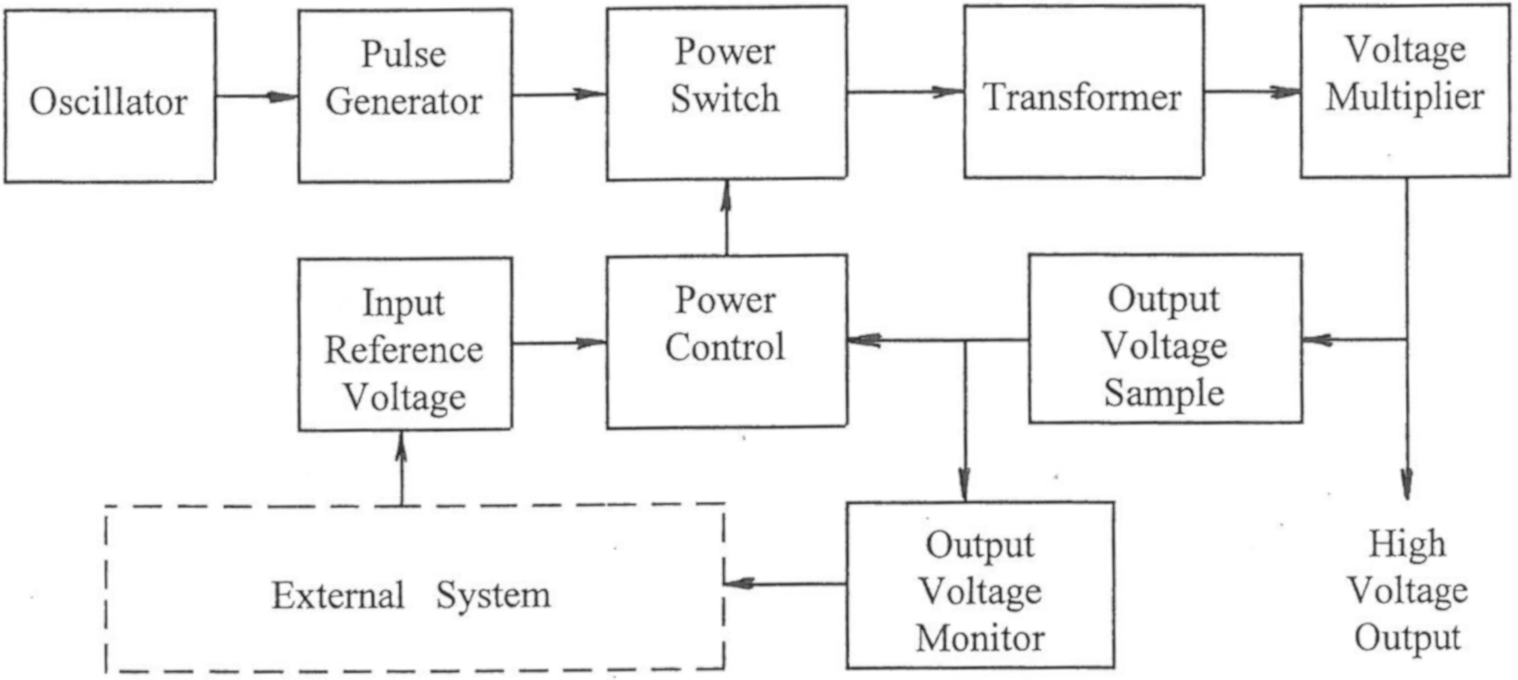
\includegraphics[width=.9\textwidth]{figures/block-diagram.png}
\caption{Architecture of the circuit in appendix \ref{app:main-circuit}.}
\label{fig:1:architecture}
\end{figure}





%----------------------------------------------------------------------------------------
%	THE OVER ALL BLOCK DIAGRAM.
%----------------------------------------------------------------------------------------
\subsection{The over-all block diagram}






%----------------------------------------------------------------------------------------
%	REQUIREMENTS.
%	
% 	INFO transistors (FIG 19 & 20): http://www.industrial-electronics.com/DC_pwr_3.html
%----------------------------------------------------------------------------------------
\subsection{Special voltage \& power requirements}






%----------------------------------------------------------------------------------------
%	TEST PROCEDURE.
%----------------------------------------------------------------------------------------
\subsection{Test procedure to prevent anybody touching the high voltage}









%----------------------------------------------------------------------------------------
%	PROCEDURE 2: TESTING THE INDIVIDUAL PARTS OF THE SYSTEM.
%----------------------------------------------------------------------------------------
\newpage
\section{Testing the individual parts of the system}
In this chapter the individual blocks/subsystems are tested and documented.

\subsection{Safety}
Disable the high voltage part of the circuit by disconnecting the voltage multiplying ladder from the transformer output. That is, remove capacitor C4.

\subsection{Power supply}
Connect the $\SI{5}{\volt}$ and the $\pm \SI{12}{\volt}$ supplies to the board but \textbf{NOT} the 30\,Volt supply!

%----------------------------------------------------------------------------------------
%	THE OSCILLATOR.
%----------------------------------------------------------------------------------------
\subsection{The oscillator}


\begin{figure}[H]
\centering
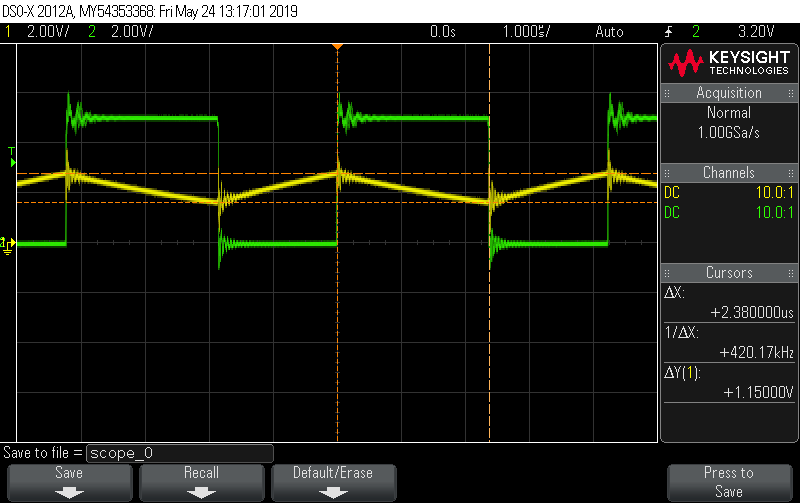
\includegraphics[width=.9\textwidth]{figures/scope_0.png}
\caption{The Schmitt trigger circuit (oscillator) with yellow being the input 'TCP' and green the output 'OSC-OP' at a random frequency.}
\label{fig:scope_0}
\end{figure}


\begin{figure}[H]
\centering
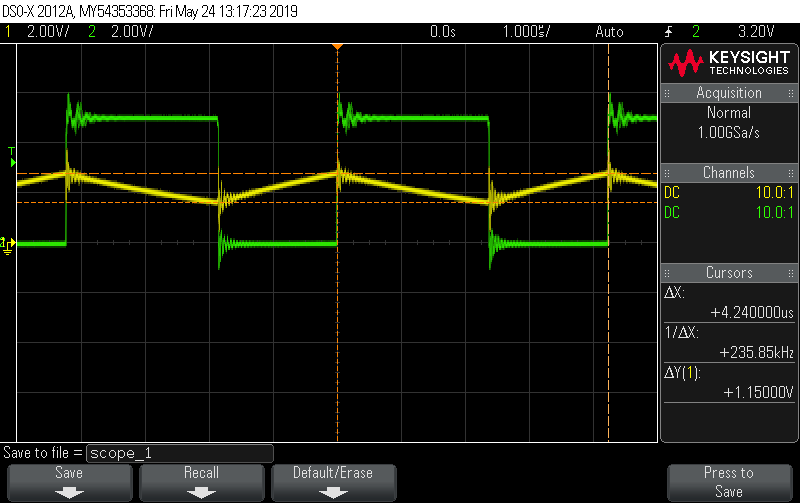
\includegraphics[width=.9\textwidth]{figures/scope_1.png}
\caption{The Schmitt trigger circuit (oscillator) with yellow being the input 'TCP' and green the output 'OSC-OP' at a random frequency.}
\label{fig:scope_1}
\end{figure}


\begin{figure}[H]
\centering
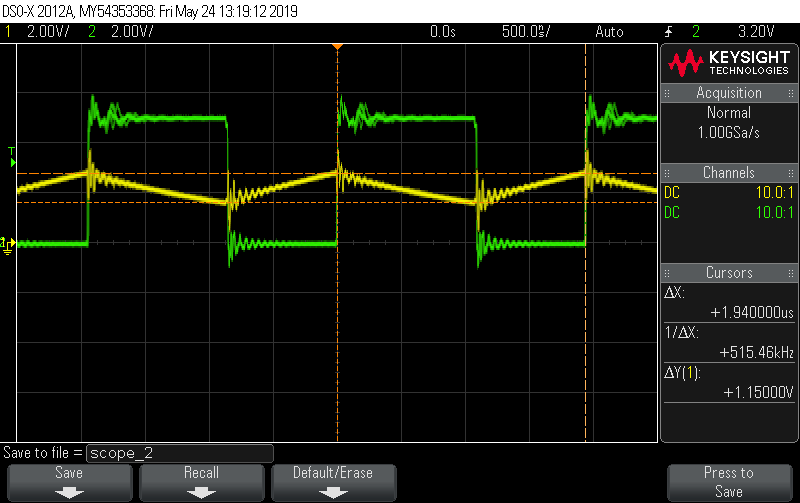
\includegraphics[width=.9\textwidth]{figures/scope_2.png}
\caption{The Schmitt trigger circuit (oscillator) with yellow being the input 'TCP' and green the output 'OSC-OP' with the maximum frequency.}
\label{fig:scope_2}
\end{figure}


\begin{figure}[H]
\centering
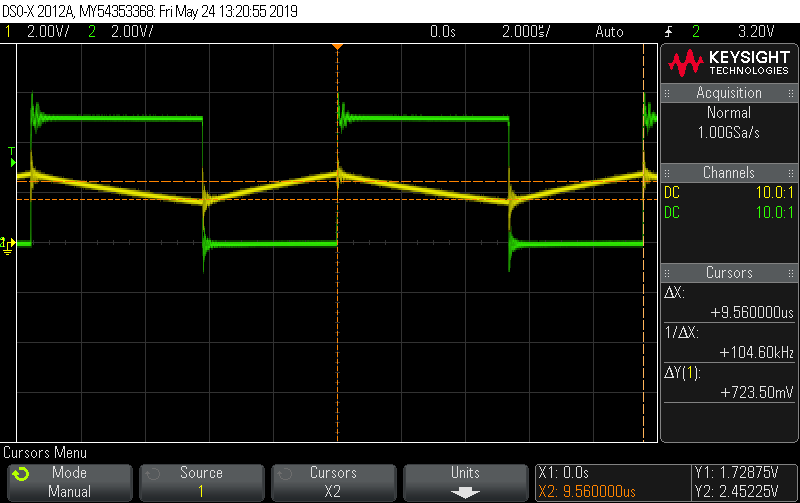
\includegraphics[width=.9\textwidth]{figures/scope_3.png}
\caption{The Schmitt trigger circuit (oscillator) with yellow being the input 'TCP' and green the output 'OSC-OP' with the minimum frequency.}
\label{fig:scope_3}
\end{figure}


%----------------------------------------------------------------------------------------
%	THE PULSE GENERATOR.
%----------------------------------------------------------------------------------------
\subsection{The pulse generator}


\begin{figure}[H]
\centering
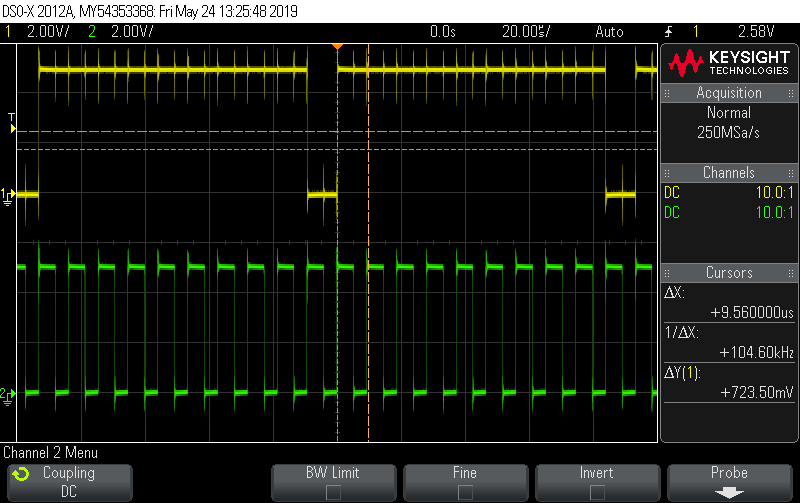
\includegraphics[width=.9\textwidth]{figures/scope_4.png}
\caption{Pulse generator circuit with yellow on 'PULSE 0' and green on 'OSC-OP', the interface between the oscillator and pulse generator.}
\label{fig:scope_4}
\end{figure}


\begin{figure}[H]
\centering
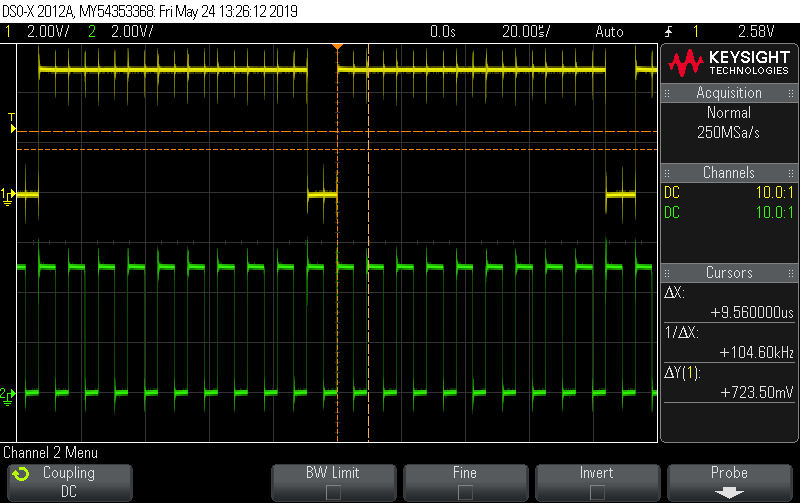
\includegraphics[width=.9\textwidth]{figures/scope_5.png}
\caption{Pulse generator circuit with yellow on 'PULSE 1' and green on 'OSC-OP', the interface between the oscillator and pulse generator.}
\label{fig:scope_5}
\end{figure}


\begin{figure}[H]
\centering
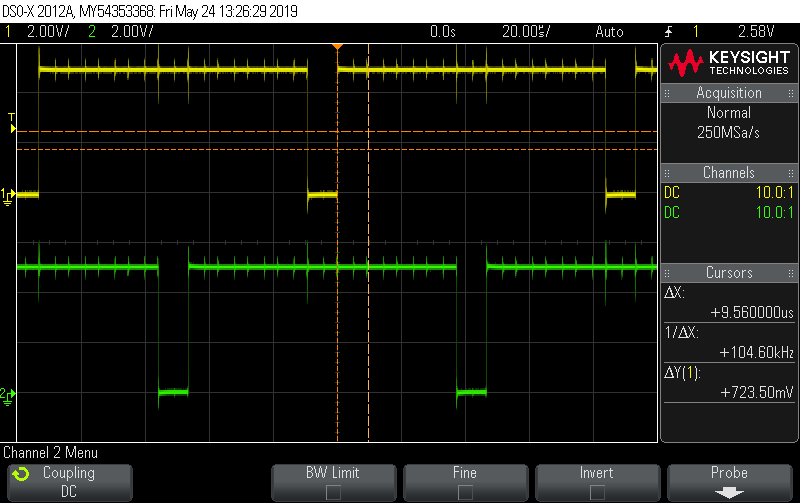
\includegraphics[width=.9\textwidth]{figures/scope_6.png}
\caption{Pulse generator circuit with yellow on 'PULSE 1' and green on 'PULSE 0'. It can be seen that the timing between these pulses is equal.}
\label{fig:scope_6}
\end{figure}


%----------------------------------------------------------------------------------------
%	OUTPUT VOLTAGE SAMPLE AND OUTPUT VOLTAGE MONITOR.
%----------------------------------------------------------------------------------------
\subsection{Output voltage sample \& voltage monitor}


\begin{figure}[H]
\centering
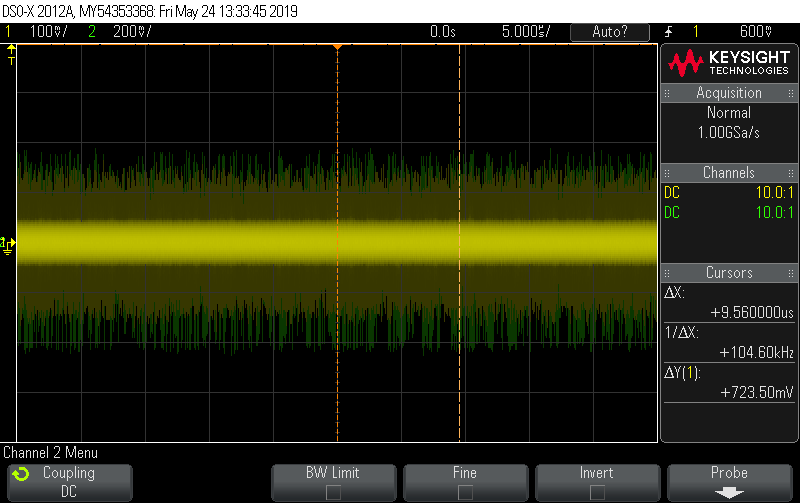
\includegraphics[width=.9\textwidth]{figures/scope_7.png}
\caption{The output voltage sampler with the input in yellow being 'FEEDBACK I/P' and the output in green being 'OP-AMP O/P'. The 'FEEDBACK I/P' is here $\approx \SI{0}{\volt}$.}
\label{fig:scope_7}
\end{figure}


\begin{figure}[H]
\centering
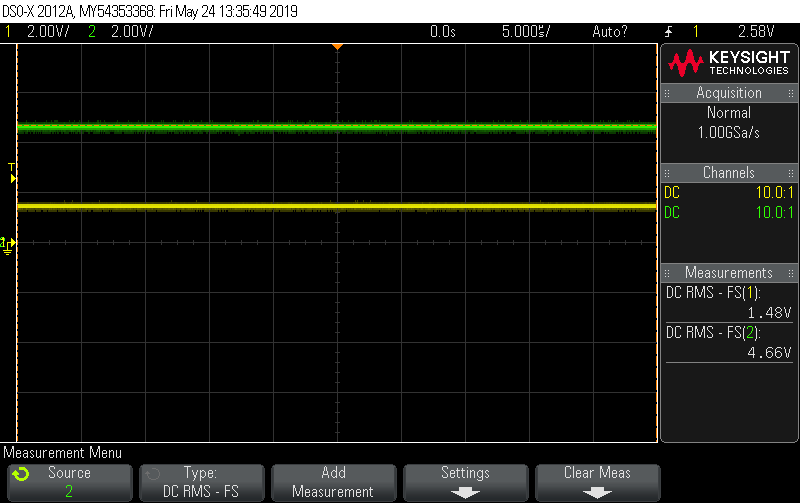
\includegraphics[width=.9\textwidth]{figures/scope_8.png}
\caption{The output voltage sampler with the input in yellow being 'FEEDBACK I/P' and the output in green being 'OP-AMP O/P'. The 'FEEDBACK I/P' is here $\approx \SI{1.5}{\volt}$.}
\label{fig:scope_8}
\end{figure}


\begin{figure}[H]
\centering
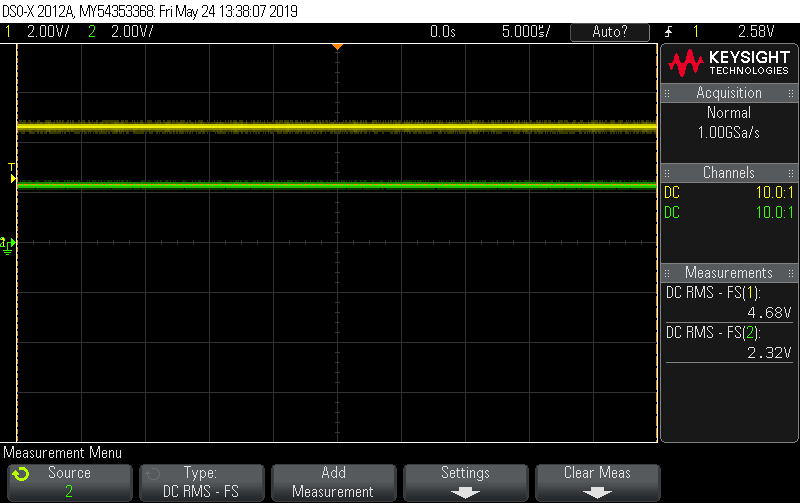
\includegraphics[width=.9\textwidth]{figures/scope_10.png}
\caption{The output voltage monitor with the input in yellow being 'OP-AMP O/P' and the output in green being 'J8 connector' or 'high voltage monitor'. The gain has been set to minimal with R16.}
\label{fig:scope_10}
\end{figure}


\begin{figure}[H]
\centering
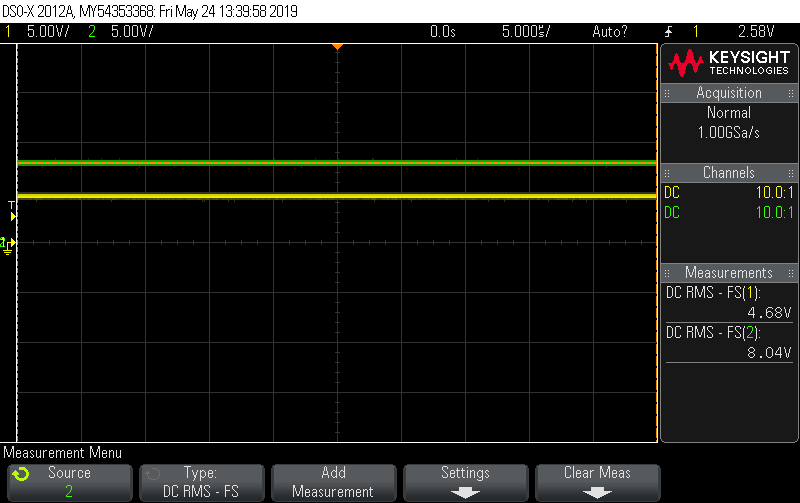
\includegraphics[width=.9\textwidth]{figures/scope_11.png}
\caption{The output voltage monitor with the input in yellow being 'OP-AMP O/P' and the output in green being 'J8 connector' or 'high voltage monitor'. The gain has been set to maximal with R16.}
\label{fig:scope_11}
\end{figure}


\begin{figure}[H]
\centering
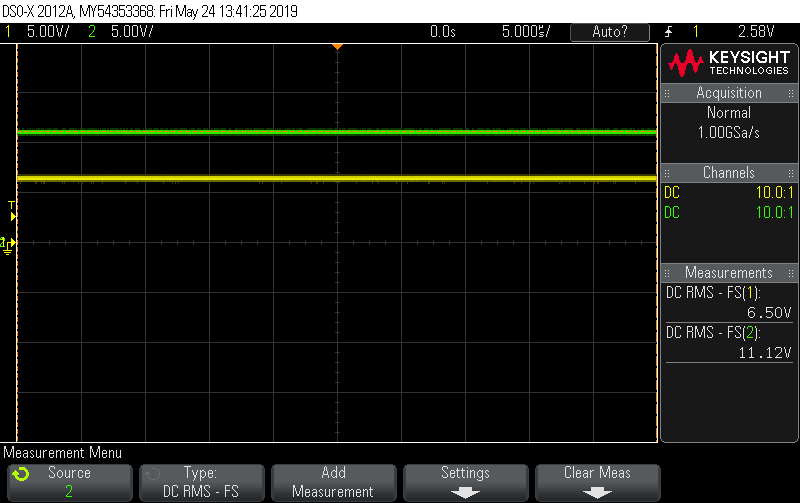
\includegraphics[width=.9\textwidth]{figures/scope_12.png}
\caption{The output voltage monitor with the input in yellow being 'OP-AMP O/P' and the output in green being 'J8 connector' or 'high voltage monitor'. The 'FEEDBACK I/P' voltage has been increased to $\SI{2}{\volt}$.}
\label{fig:scope_12}
\end{figure}


%----------------------------------------------------------------------------------------
%	INPUT REFERENCE VOLTAGE AND POWER CONTROL.
%----------------------------------------------------------------------------------------
\subsection{Input reference voltage \& power control}


\begin{figure}[H]
\centering
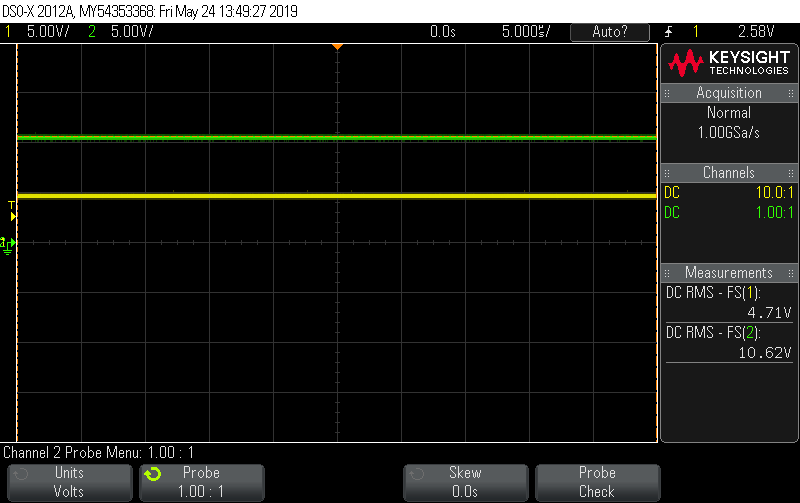
\includegraphics[width=.9\textwidth]{figures/scope_13.png}
\caption{Input reference voltage with variable resistor R6 on 100\%. The input 'OP-AMP O/P' in yellow and the output 'TP3' (input power control) in green.}
\label{fig:scope_13}
\end{figure}


\begin{figure}[H]
\centering
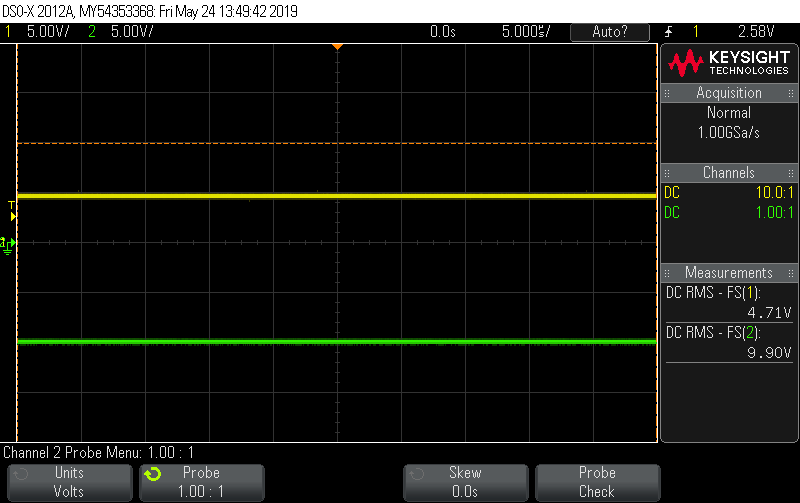
\includegraphics[width=.9\textwidth]{figures/scope_14.png}
\caption{Input reference voltage with variable resistor R6 on 0\%. The input 'OP-AMP O/P' in yellow and the output 'TP3' (input power control) in green.}
\label{fig:scope_14}
\end{figure}


\begin{figure}[H]
\centering
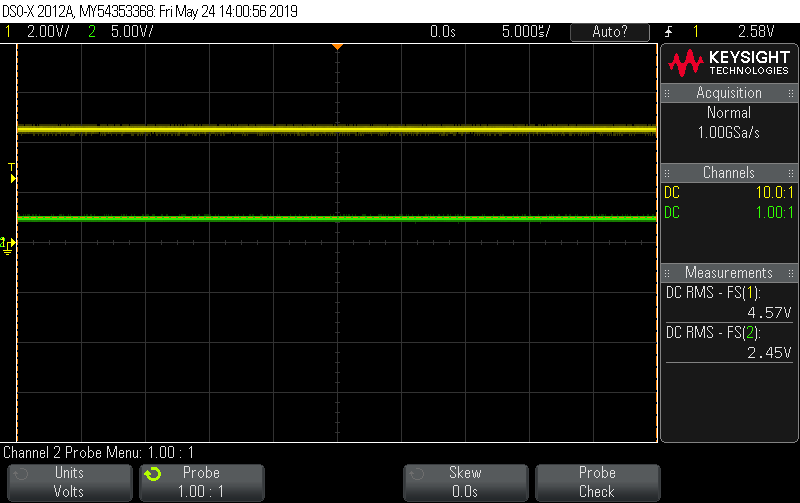
\includegraphics[width=.9\textwidth]{figures/scope_15.png}
\caption{Input reference voltage of $\SI{2.45}{\volt}$, measured in green at the positive input of the op-amp U3A. The input voltage on the negative input 'OP-AMP O/P' is $\SI{4.6}{\volt}$. The output 'TP3' is shown in yellow. It can be seen that the gain is approximately 1.}
\label{fig:scope_15}
\end{figure}


%----------------------------------------------------------------------------------------
%	POWER CONTROL AND POWER SWITCH.
%----------------------------------------------------------------------------------------
\subsection{Power control \& power switch}


\begin{figure}[H]
\centering
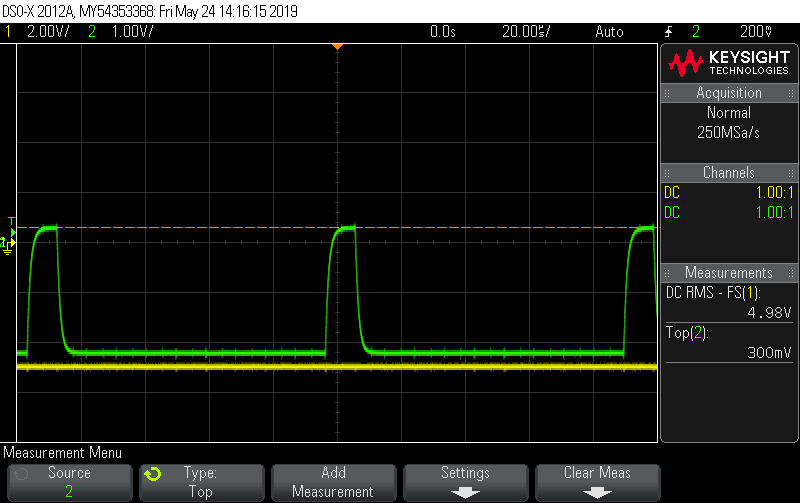
\includegraphics[width=.9\textwidth]{figures/scope_16.png}
\caption{In yellow the input 'TP3' of the power control is shown. In green the output 'TP2' from the pulse generators towards the input of the power control is shown. The voltage does of 'TP2' does not get above $\SI{0.7}{\volt}$ and thus the transistors Q1 and Q2 are inactive.}
\label{fig:scope_16}
\end{figure}


\begin{figure}[H]
\centering
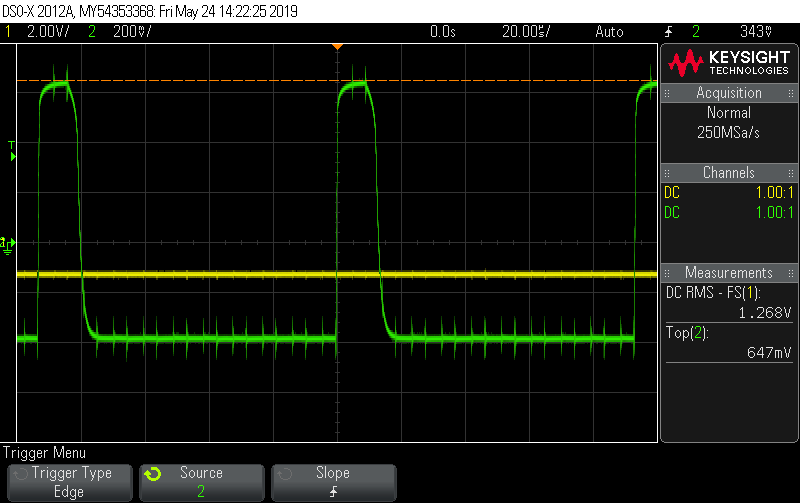
\includegraphics[width=.9\textwidth]{figures/scope_17.png}
\caption{In yellow the input 'TP3' of the power control is shown. In green the output 'TP2' from the pulse generators towards the input of the power control is shown. The reference voltage is increased just over the boundary in order to get the 'TP2' (green) above the $\SI{0.7}{\volt}$ needed to let the diodes D1 and D3 be sperred and the transistors Q1 and Q2 be enabled.}
\label{fig:scope_17}
\end{figure}


\begin{figure}[H]
\centering
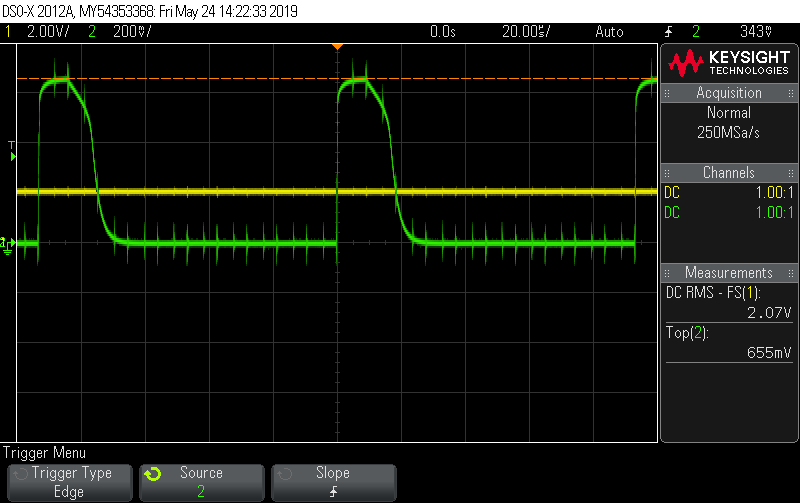
\includegraphics[width=.9\textwidth]{figures/scope_18.png}
\caption{In yellow the input 'TP3' of the power control is shown. In green the output 'TP2' from the pulse generators towards the input of the power control is shown. The reference voltage is further increased, it can be seen that the enable period gets larger.}
\label{fig:scope_18}
\end{figure}


%----------------------------------------------------------------------------------------
%	POWER SWITCH AND TRANSFORMER.
%----------------------------------------------------------------------------------------
\subsection{Power switch \& transformer}


\begin{figure}[H]
\centering
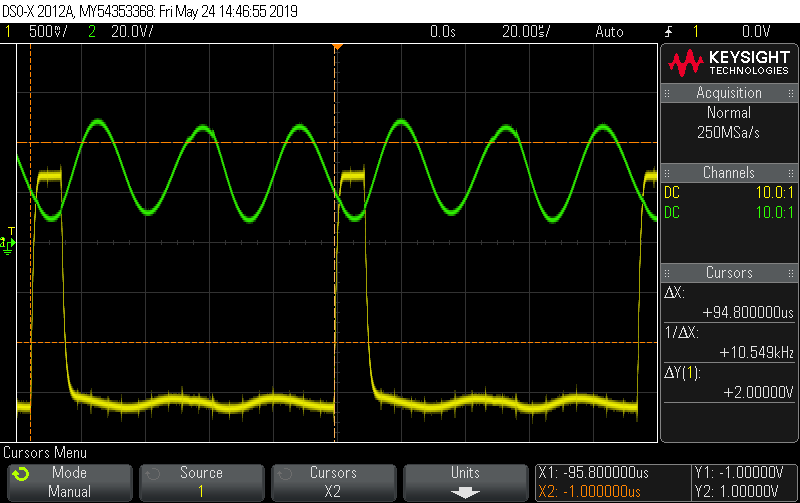
\includegraphics[width=.9\textwidth]{figures/scope_19.png}
\caption{In yellow the input 'TP2' to the power switch is shown and in green the output 'TP1' of the switch, controlling the transformer. It can be seen that the transformer is in resonance.}
\label{fig:scope_19}
\end{figure}







%----------------------------------------------------------------------------------------
%	PROCEDURE 3: HIGH VOLTAGE SYSTEM TEST.
%----------------------------------------------------------------------------------------
\newpage
\section{High voltage system test}
In this chapter the high voltage power supply has been tested and documented.

\subsection{Initial Conditions}
Follow the procedure to make the board ready for the high voltage system test:
\begin{enumerate}
	\item Turn all the power supplies to the board off.
	\item Remove the connection to the feedback pin between the resistors of $\SI{220}{\kilo\ohm}$ and $\SI{500}{\mega\ohm}$. 
	\item Replace the capacitor ($C4$) between the transformer and the voltage cascade.
	\item The rest of the settings should be the same as is in question 2.8.
	\item Turn on the $\SI{5}{\volt}$ and $\pm\SI{12}{\volt}$ power supplies.
\end{enumerate}

%----------------------------------------------------------------------------------------
%	INITIAL TEST.
%----------------------------------------------------------------------------------------
\subsection{Initial test}


\begin{figure}[H]
\centering
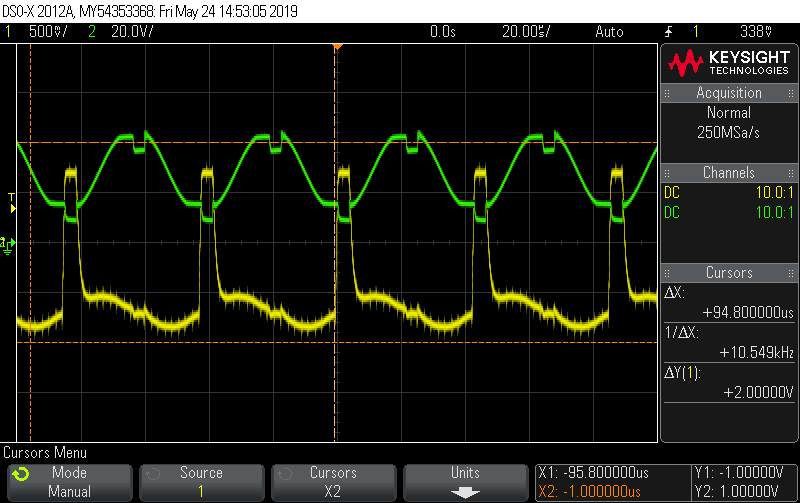
\includegraphics[width=.9\textwidth]{figures/scope_20.png}
\caption{High voltage output is connected. In yellow the input 'TP2' to the power switch is shown and in green the output 'TP1' of the switch, controlling the transformer. It can be seen that the transformer is in resonance.}
\label{fig:scope_20}
\end{figure}


We had an ugly signal, the high voltage output was 3176\,V


In order to get this output, we had to re-adjust the clock frequency of the oscillator 'CLK'.


The high voltage output voltage then increased to 3225\,V.


%----------------------------------------------------------------------------------------
%	VARIATION OF THE OUTPUT VOLTAGE.
%----------------------------------------------------------------------------------------
\subsection{Variation of the output voltage}


\begin{figure}[H]
\centering
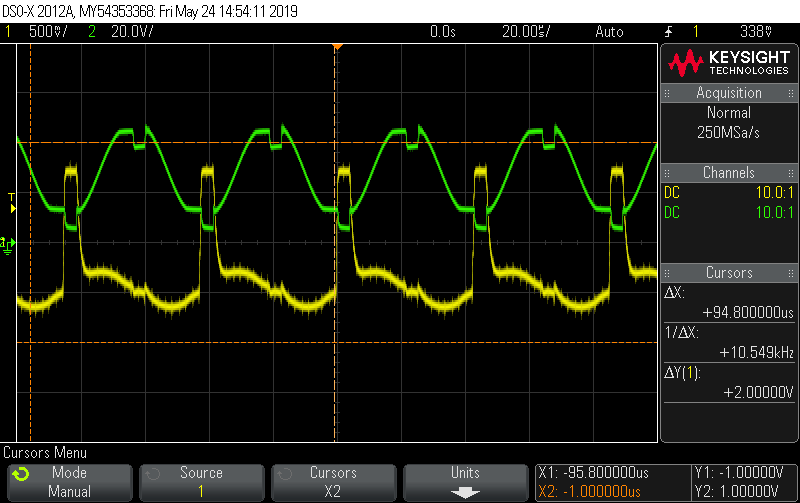
\includegraphics[width=.9\textwidth]{figures/scope_21.png}
\caption{In yellow the input 'TP2' to the power switch is shown and in green the output 'TP1' of the switch, controlling the transformer. The reference voltage has been increased to get the maximum high voltage output ($\SI{3759}{\volt}$).}
\label{fig:scope_21}
\end{figure}


\begin{figure}[H]
\centering
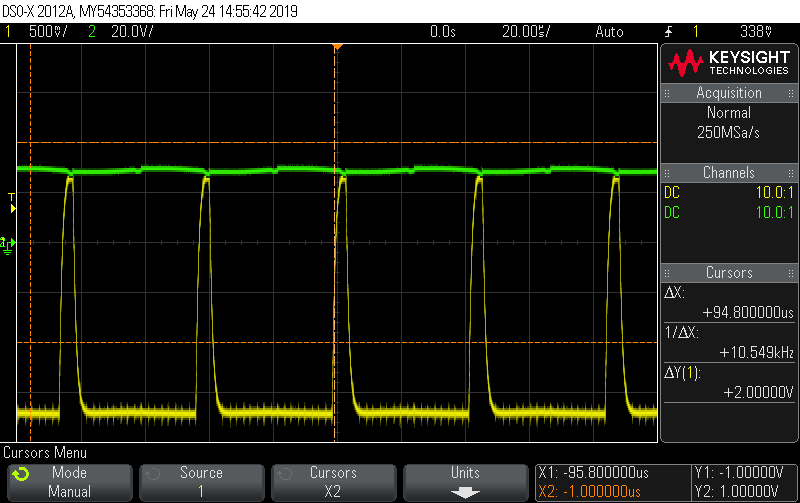
\includegraphics[width=.9\textwidth]{figures/scope_22.png}
\caption{In yellow the input 'TP2' to the power switch is shown and in green the output 'TP1' of the switch, controlling the transformer. The reference voltage has been decreased to get the minimum high voltage output ($\SI{157.7}{\volt}$).}
\label{fig:scope_22}
\end{figure}





%----------------------------------------------------------------------------------------
%	RESULTS/ CONCLUSION.
%----------------------------------------------------------------------------------------
\newpage
%----------------------------------------------------------------------------------------
%	RESULTS/ COMPARISON/ CONCLUSION.
%----------------------------------------------------------------------------------------
\section{Conclusion}









%----------------------------------------------------------------------------------------
%	APPENDICES.
%----------------------------------------------------------------------------------------
\newpage				% Start at new page.
\begin{appendices}
\part*{Appendices}
\etoctoccontentsline*{appendixplaceholder}{Appendices}{-1}
\vspace{-1cm}
\renewcommand{\contentsname}{}
\localtableofcontents*


    %------------------------------------------------------------------------------------
    %	APPENDIX: MAIN CIRCUIT.
    %------------------------------------------------------------------------------------
    \begin{landscape}
    \section{\label{app:main-circuit}Main electrical circuit of Lab 4}
    \begin{figure}[h!]
	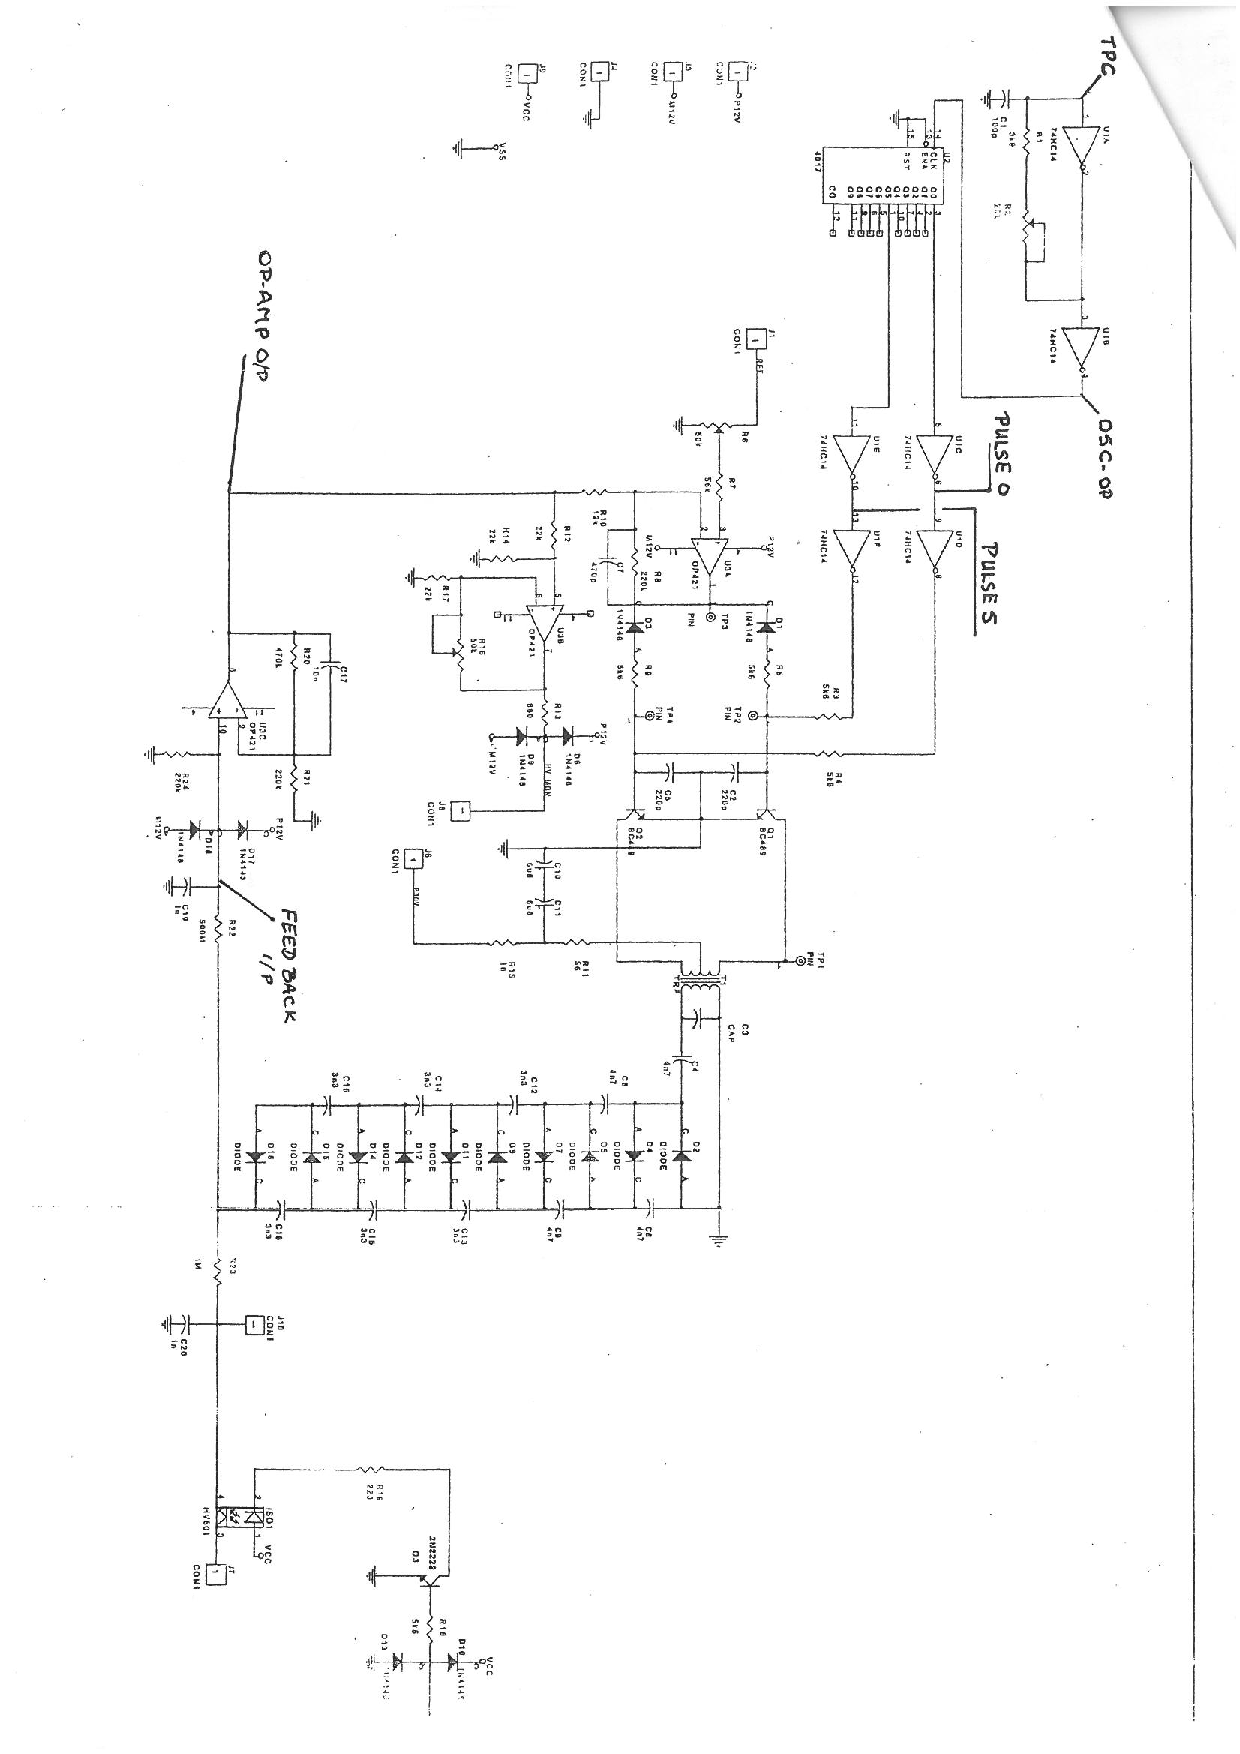
\includepdf[pages=1, angle=180]{figures/Lab4-schema.pdf}
	\end{figure}
	\end{landscape}

\end{appendices}



\end{document}


